\documentclass{article}

    \usepackage{fancyhdr}
    \usepackage{extramarks}
    \usepackage{amsmath}
    \usepackage{amsthm}
    \usepackage{amsfonts}
    \usepackage{tikz}
    \usepackage{amssymb}
    \usepackage{subcaption}
    \usepackage{blkarray}
    \usetikzlibrary{arrows, automata}
    \usepackage{forest}

    


    \usepackage{enumitem}

    \setlist[enumerate,1]{start=0} % only outer nesting level


    \usepackage{tabulary}

\usepackage[newcommands]{ragged2e}

    \usetikzlibrary{trees}

    \newcommand{\question}{\textbf{Question:}}
    \newcommand{\answer}{\textbf{Answer:}}

    


    \usetikzlibrary{decorations.markings}
    \tikzstyle{vertex}=[circle, draw, inner sep=0pt, minimum size=6pt]
    \newcommand{\vertex}{\node[vertex]}

    
    \usepackage{amsmath}
    \usepackage{algorithm}
    \usepackage[noend]{algpseudocode}
    \usepackage[utf8]{inputenc}
    \usepackage{enumerate}
    \usepackage{geometry}
    \usepackage{mathtools}
    \usepackage{parskip}
    \usepackage{xifthen, xparse}
    
    \algdef{SE}[SUBALG]{Indent}{EndIndent}{}{\algorithmicend\ }%
    \algtext*{Indent}
    \algtext*{EndIndent}
    
    
    
    \usetikzlibrary{automata,positioning}
    
    %
    % Basic Document Settings
    %
    
    \topmargin=-0.45in
    \evensidemargin=0in
    \oddsidemargin=0in
    \textwidth=6.5in
    \textheight=9.0in
    \headsep=0.25in
    
    \linespread{1.1}
    
    \pagestyle{fancy}
    \lhead{\hmwkAuthorName}
    \chead{\hmwkClass\ \hmwkTitle}
    \rhead{\firstxmark}
    \lfoot{\lastxmark}
    \cfoot{\thepage}
    
    \renewcommand\headrulewidth{0.4pt}
    \renewcommand\footrulewidth{0.4pt}
    
    \setlength\parindent{0pt}
    
    %
    % Create Problem Sections
    %
    
    \newcommand{\enterProblemHeader}[1]{
        \nobreak\extramarks{}{Problem \arabic{#1} continued on next page\ldots}\nobreak{}
        \nobreak\extramarks{Problem \arabic{#1} (continued)}{Problem \arabic{#1} continued on next page\ldots}\nobreak{}
    }
    
    \newcommand{\exitProblemHeader}[1]{
        \nobreak\extramarks{Problem \arabic{#1} (continued)}{Problem \arabic{#1} continued on next page\ldots}\nobreak{}
        \stepcounter{#1}
        \nobreak\extramarks{Problem \arabic{#1}}{}\nobreak{}
    }
    
    \newcommand\rowop[1]{\scriptstyle\smash{\xrightarrow[\vphantom{#1}]{\mkern-4mu#1\mkern-4mu}}}
    
    \DeclareDocumentCommand\converttorows%
    {>{\SplitList{,}}m}%
    {\ProcessList{#1}{\converttorow}}
    \NewDocumentCommand{\converttorow}{m}
    {\ifthenelse{\isempty{#1}}{}{\rowop{#1}}\\}
    
    \DeclareDocumentCommand \rowops{m}
    {\;
     \begin{matrix}
    \converttorows {#1}
     \end{matrix}
     \; }
    
    \setcounter{secnumdepth}{0}
    \newcounter{partCounter}
    \newcounter{homeworkProblemCounter}
    \setcounter{homeworkProblemCounter}{1}
    \nobreak\extramarks{Problem \arabic{homeworkProblemCounter}}{}\nobreak{}
    
    %
    % Homework Problem Environment
    %
    % This environment takes an optional argument. When given, it will adjust the
    % problem counter. This is useful for when the problems given for your
    % assignment aren't sequential. See the last 3 problems of this template for an
    % example.
    %
    \newenvironment{homeworkProblem}[1][-1]{
        \ifnum#1>0
            \setcounter{homeworkProblemCounter}{#1}
        \fi
        \section{Problem \arabic{homeworkProblemCounter}}
        \setcounter{partCounter}{1}
        \enterProblemHeader{homeworkProblemCounter}
    }{
        \exitProblemHeader{homeworkProblemCounter}
    }
    
    %
    % Homework Details
    %   - Title
    %   - Due date
    %   - Class
    %   - Section/Time
    %   - Instructor
    %   - Author
    %
    
    \newcommand{\hmwkTitle}{SOFTENG250 Assignment \#6}
    \newcommand{\hmwkClass}{D.S. and Algorithms}
    \newcommand{\hmwkAuthorName}{\textbf{Nisarag Bhatt}}
    
    
    %
    % Title Page
    %
    
    \title{
        \vspace{2in}
        \textmd{\textbf{\hmwkClass:\ \hmwkTitle}}\\
        \textmd{\textbf{ID Number: \idnumber}}\\
        \textmd{\textbf{UPI: \upi}}\\
        \vspace{3in}
    }
    
    \author{\hmwkAuthorName}
    \date{}
    
    \renewcommand{\part}[1]{\textbf{\large Part \Alph{partCounter}}\stepcounter{partCounter}\\}
    
    %
    % Various Helper Commands
    %
    
    % Useful for algorithms
    \newcommand{\alg}[1]{\textsc{\bfseries \footnotesize #1}}
    
    % For derivatives
    \newcommand{\deriv}[1]{\frac{\mathrm{d}}{\mathrm{d}x} (#1)}
    
    % For partial derivatives
    \newcommand{\pderiv}[2]{\frac{\partial}{\partial #1} (#2)}
    
    % Integral dx
    \newcommand{\dx}{\mathrm{d}x}
    
    % Alias for the Solution section header
    \newcommand{\solution}{\textbf{\large Solution}}
    
    % Probability commands: Expectation, Variance, Covariance, Bias
    \newcommand{\E}{\mathrm{E}}
    \newcommand{\Var}{\mathrm{Var}}
    \newcommand{\Cov}{\mathrm{Cov}}
    \newcommand{\Bias}{\mathrm{Bias}}
    
    \begin{document}
    
    
    \pagebreak
    
    \begin{homeworkProblem}

        \question
        
        Suppose $S=\{a, b, c, d, e, g, i, j\}$ , where the frequencies are $fa= 0.25, fb= 0.15, fc= 0.16, fd= 0.14, fe= 0.15, fg= 0.05, fi= 0.04, fj= 0.06$. Build an optimal prefix code for this data.

        \answer

        Consider sorting this data by increasing frequency so we get the following Char, Frequency and Prefix Codes by Huffman Algorithm:  
        
        \begin{tabular}{ l | c | r }
            Char & Frequency & Prefix Code  \\
            \hline
            $i$ & $0.04$ & $\gamma(i) = 11110$ \\
            $g$ & $0.05$ & $\gamma(g) = 11111$ \\
            $j$ & $0.06$ & $\gamma(j) = 1110$  \\
            $d$ & $0.14$ & $\gamma(d) = 110$  \\ 
            $e$ & $0.15$ & $\gamma(e) = 100$  \\ 
            $b$ & $0.15$ & $\gamma(b) = 101$  \\ 
            $c$ & $0.16$ & $\gamma(c) = 00$ \\ 
            $a$ & $0.25$ & $\gamma(a) = 01$ \\ 
        \end{tabular}

        This is the tree we get from the huffman algorithm

        \begin{center}
            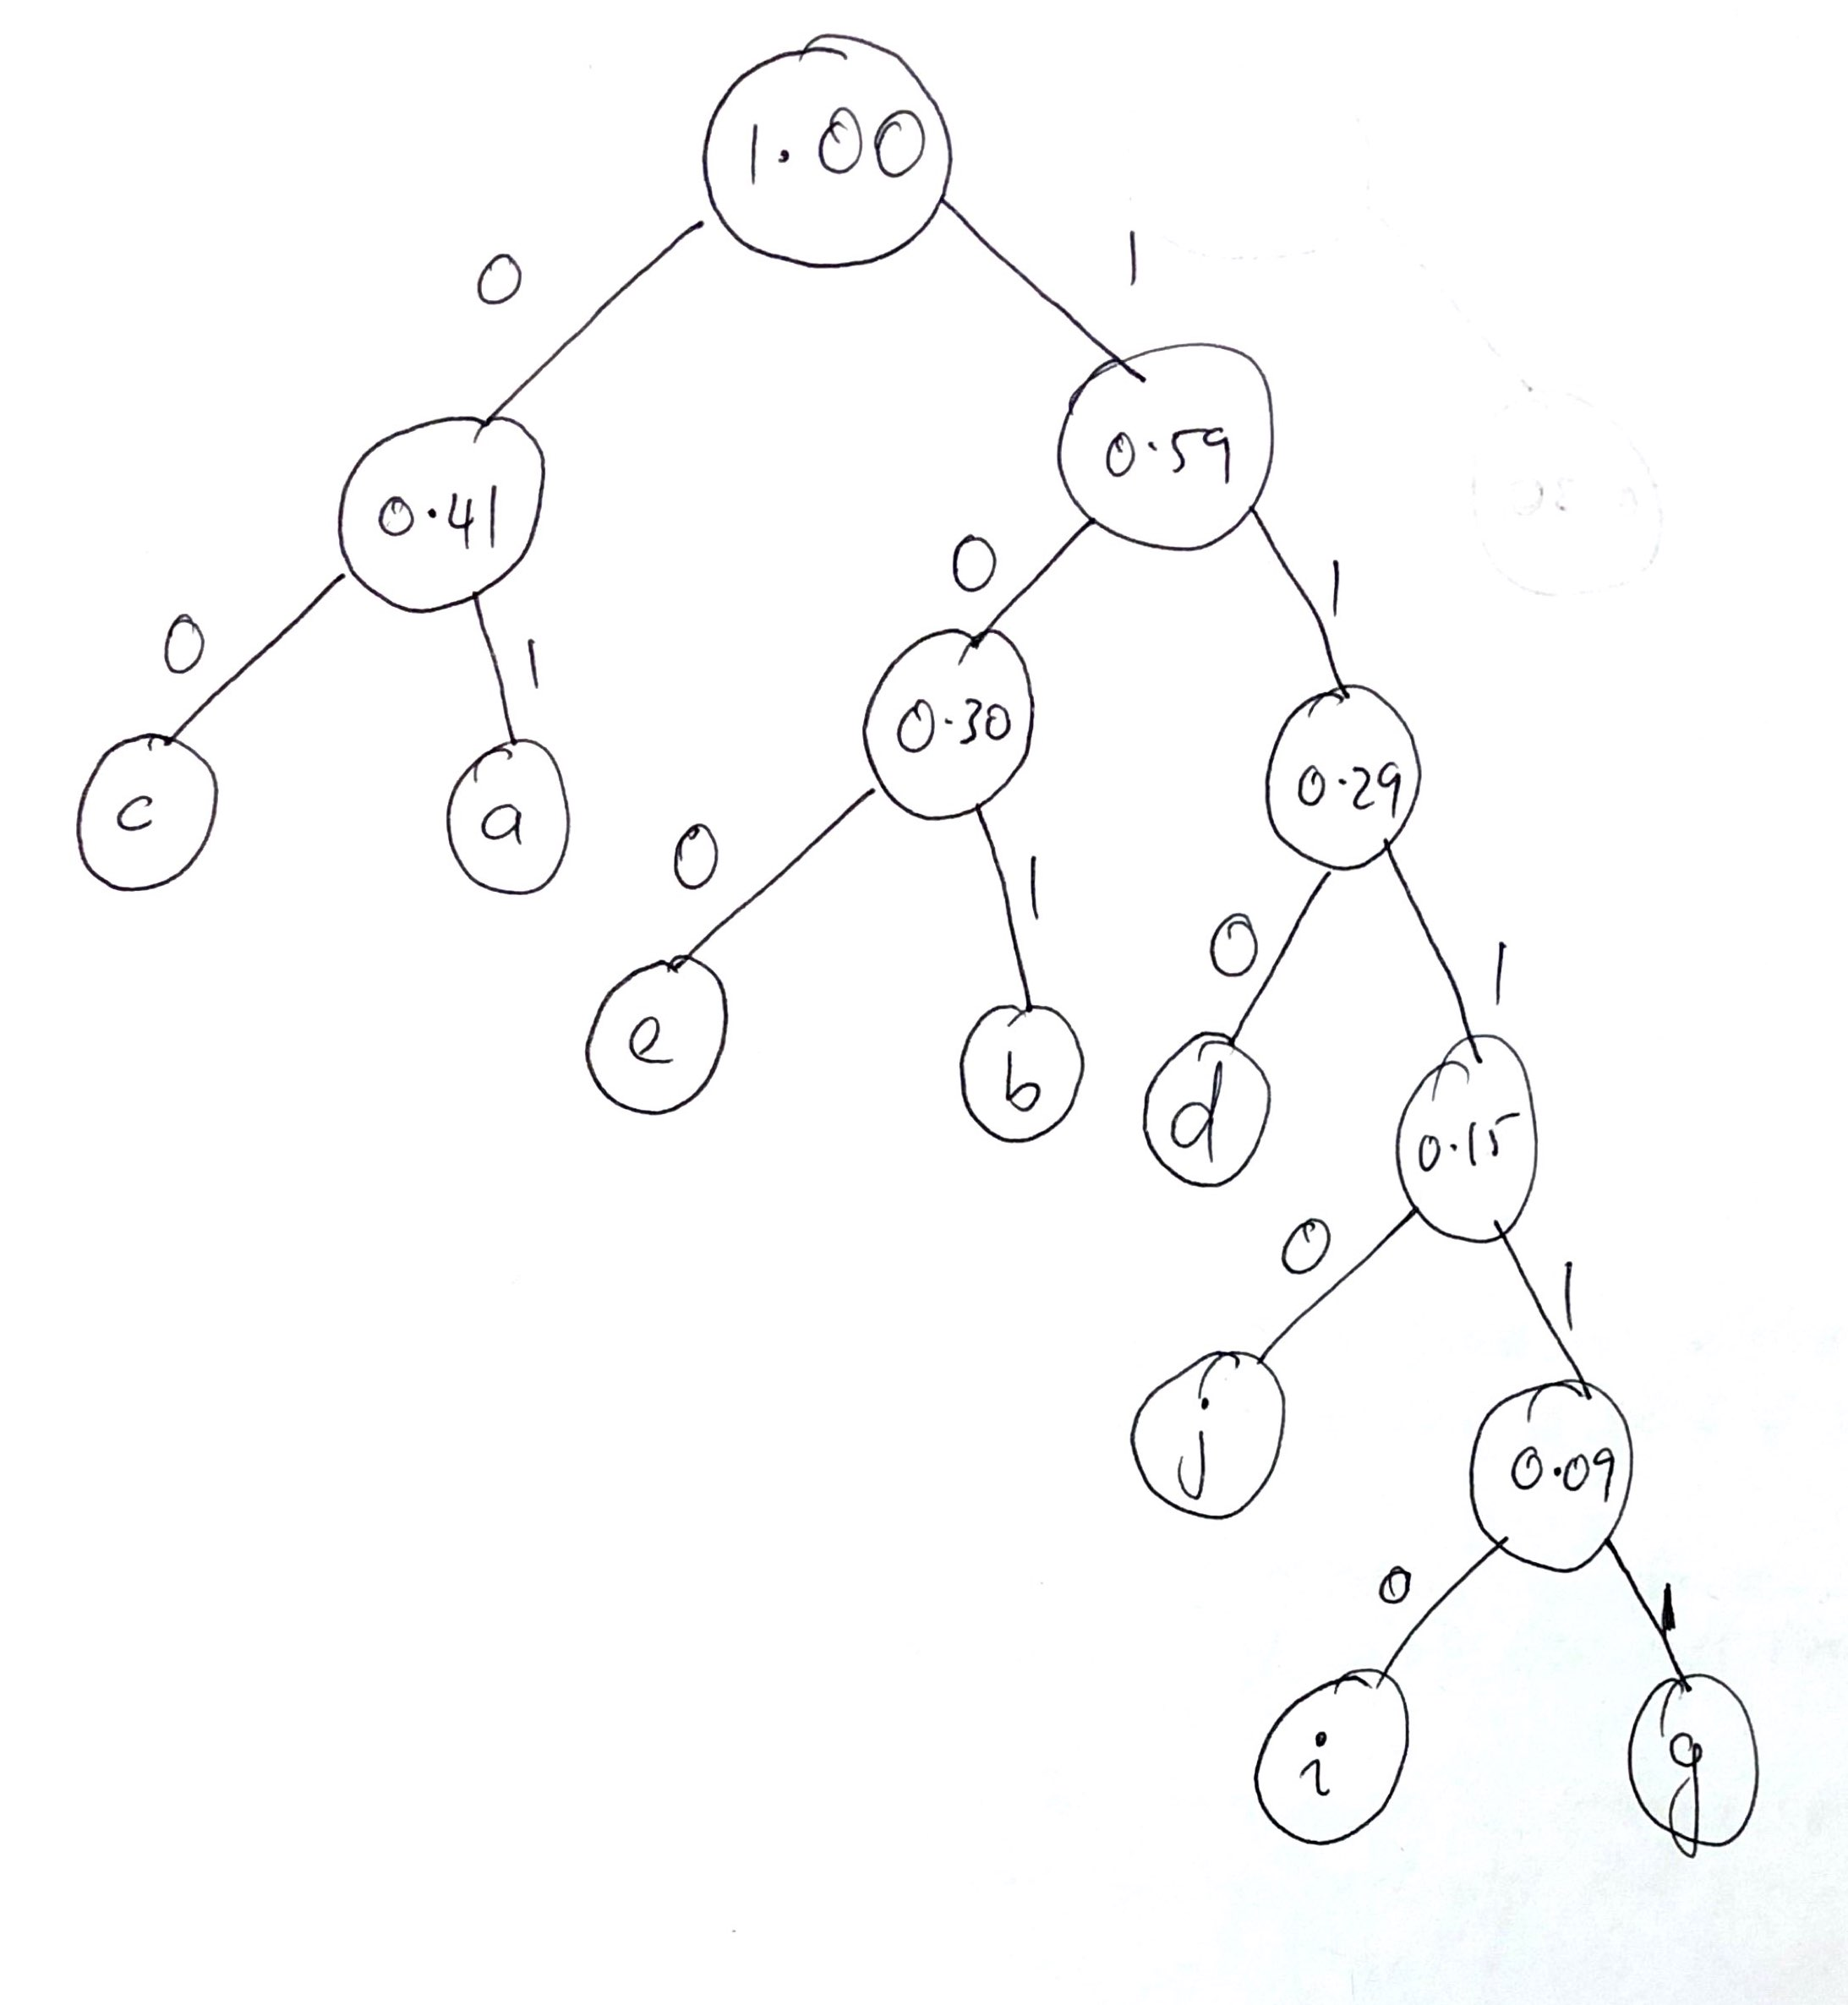
\includegraphics[scale = 0.15]{tree.jpg}
        \end{center}  
    
    \end{homeworkProblem}

    \begin{homeworkProblem}
        \question 

        For each of the following recurrence relations find the general pattern formula and find the running time $T(n)$ of the algorithm given by the recurrence relations:

        \answer 

        $(a)$ \begin{align*}
            T(n) &\leq 3T(n/2) + Cn  \\
            & \leq 9T(n/4) + 2Cn \\ 
            & \leq 27T(n/8) + 3Cn \\
            & \leq 3^k T(n/2^k) + kCn ~~~~~~~~~~ n/2^k = 1 ~~ \text{at termination} \implies k = \log_2(n)~~ \text{and} ~~T(1)=1 \\ 
            & \leq 3^{\log_2(n)} + Cn \cdot \log_2(n) \\
            & \leq n^{\log_2(3)} + Cn \cdot \log_2(n) \\
            T(n) & = \mathcal{O}(n^{1.585})
        \end{align*}

        $(b)$ \begin{align*}
            T(n) &\leq 2T(n/3) + C  \\
            & \leq 4T(n/9) + 2C \\ 
            & \leq 8T(n/27) + 3C \\
            & \leq 2^k T(n/3^k) + kC ~~~~~~~~~~ n/3^k = 1 ~~ \text{at termination} \implies k = \log_3(n)~~ \text{and} ~~T(1)=1 \\ 
            & \leq 2^{\log_3(n)} + C \cdot \log_3(n) \\
            & \leq n^{\log_3(2)} + C \cdot \log_3(n) \\
            T(n) & = \mathcal{O}(n^{0.63})
        \end{align*}

        $(c)$ \begin{align*}
            T(n) &\leq 5T(n/4) + Cn  \\
            & \leq 25T(n/16) + 2Cn \\ 
            & \leq 125T(n/64) + 3Cn \\
            & \leq 5^k T(n/4^k) + kCn ~~~~~~~~~~ n/4^k = 1 ~~ \text{at termination} \implies k = \log_4(n)~~ \text{and} ~~T(1)=1 \\ 
            & \leq 5^{\log_4(n)} + Cn \cdot \log_4(n) \\
            & \leq n^{\log_4(5)} + Cn \cdot \log_4(n) \\
            T(n) & = \mathcal{O}(n^{1.16})
        \end{align*}

        $(d)$ \begin{align*}
            T(n) &\leq 2T(n/2) + C  \\
            & \leq 4T(n/4) + 2C \\ 
            & \leq 8T(n/8) + 3C \\
            & \leq 2^k T(n/2^k) + kC ~~~~~~~~~~ n/2^k = 1 ~~ \text{at termination} \implies k = \log_2(n)~~ \text{and} ~~T(1)=1 \\ 
            & \leq 2^{\log_2(n)} + C \cdot \log_2(n) \\
            & \leq n + C \cdot \log_2(n) \\
            T(n) & = \mathcal{O}(n)
        \end{align*}

        $(e)$ \begin{align*}
            T(n) &\leq 9T(n/3) + Cn^2  \\
            & \leq 81T(n/9) + 2Cn^2 \\ 
            & \leq 729T(n/27) + 3Cn^2 \\
            & \leq 9^k T(n/3^k) + kCn^2 ~~~~~~~~~~ n/3^k = 1 ~~ \text{at termination} \implies k = \log_3(n)~~ \text{and} ~~T(1)=1 \\ 
            & \leq 9^{\log_3(n)} + Cn^2 \cdot \log_3(n) \\
            & \leq n^{\log_3(9)} + Cn^2 \cdot \log_3(n) \\
            & \leq n^2 + Cn^2 \cdot \log_3(n) \\
            T(n) & = \mathcal{O}(n^{2} \log_3(n)) = \mathcal{O}(n^2 \log(n))
        \end{align*}

        $(f)$ \begin{align*}
            T(n) &\leq 8T(n/2) + Cn^3  \\
            & \leq 64T(n/4) + 2Cn^3 \\ 
            & \leq 512T(n/8) + 3Cn^3 \\
            & \leq 8^k T(n/2^k) + kCn^3 ~~~~~~~~~~ n/2^k = 1 ~~ \text{at termination} \implies k = \log_2(n)~~ \text{and} ~~T(1)=1 \\ 
            & \leq 8^{\log_2(n)} + Cn^3 \cdot \log_2(n) \\
            & \leq n^{\log_2(8)} + Cn^3 \cdot \log_2(n) \\
            & \leq n^{3} + Cn^3 \cdot \log_3(n) \\
            T(n) & = \mathcal{O}(n^3 \log_3(n)) = \mathcal{O}(n^3 \log(n))
        \end{align*}
    \end{homeworkProblem}

    \pagebreak

    \begin{homeworkProblem}

        \question 
        
        Say that an array $A$ with $n$ elements has a majority element if more than half of its entries are the same. The elements of the arrays are not necessarily comparable (that is you cant ask the questions of the type $A(i) \leq A(j)$?). However, assume that you can ask the questions of the type $A(i) =A(j)$ in constant time. 
        
        Design an algorithm that tells us if $A$ has a majority element. Your algorithm should run in $\mathcal{O}(n \cdot \log(n))$ time.

        \answer 

        The whole idea of the algorithm is to Divide until you reach the base case and then Conquer up towards the required answer :
        
        Split the array recursively into halves, at the bottom layer where there are only $1$ element in the array. Return the element into the layer above where a comparison is made with the other $1$ element half.

        The comparison is as follow:

        \textbf{Case $1$}: if both halves returns an element (true) , if the elements are the same, then return this element up to the higher layer as  the majority element combined would also be a majority element in the combined array. If the elements are not the same, count the occurrence of each of the element in the array at the current layer. Return the element that has a higher count, if both count equals then return no majority.

        \textbf{Case $2$}: If exactly $1$ half returns an element (true) and the other returns no majority (false), then count the occurrence of the element, if it is greater or equal to $n/2+1$ where n is the total number of elements of the array at the layer, then the array would have a majority element else it does not.

        \textbf{Case $3$}: if both halves returns no majority (false) , then the combine array would also not have a majority element.

        Recursively run the algorithm up, and if an element is returned at the end, then the full array would have a majority element otherwise it does not. Note that String can be used as return type as it can represent both characters and integer values. By using this tree structure, the run-time of the algorithm will be O(nlogn).

        \pagebreak


    \end{homeworkProblem}
    

    \begin{homeworkProblem}


        \question 

        Solve Exercises 1 and 2 in Lecture Note 14.

        \answer 

        \textbf{Exercise 1}: Show that applying the greedy algorithm developed for the interval scheduling problem does not solve the weighted interval scheduling problem.

        Let $v_i$ represent the weight of a request $r_i$

        Consider this schedule 

        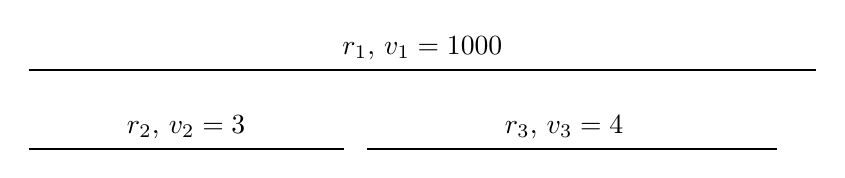
\begin{tikzpicture}
            \draw[line width=0.25mm] (0,0) -- (10,0)  node[above,xshift=-5cm] {$r_1$, $v_1 = 1000$};
            \draw[line width=0.25mm] (0,-1) -- (4.0,-1) node[above,xshift=-2cm] {$r_2$, $v_2 = 3$};
            \draw[line width=0.25mm] (4.3,-1) -- (9.5,-1) node[above,xshift=-2.7cm] {$r_3$, $v_3 = 4$};
        \end{tikzpicture}
        
        Using the greedy algorithm to select requests, the greedy algorithm would choose at each step/iteration the request that finishes first. 
        
        In the counter example above, the greedy algorithm would choose $r_2$ as it has the earliest finishing time (and eliminate $r_1$ since it is overlapping). Then, it would choose $r_3$ as that is the request that finishes next and it does not overlap with $r_2$. 
        
        The algorithm/schedule would end with a total weight of $7$. 
        
        The optimal solution would be choosing $r_1$ where the total weight would be $1000$. Therefore, the greedy algorithm does not always produce the optimal solution.

        \textbf{Excercise 2}: Consider the sequence $p(1), p(2), . . . , p(n)$.

        1. Give examples where this sequence consist of 0s only.

        In words: $r_k$ is not compatible with $r_{k-1},...,r_1$

        This usually happens when each request overlaps with all the requests before it for example:

        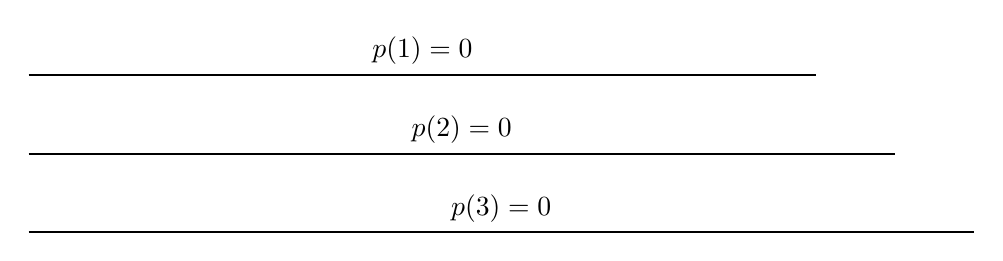
\begin{tikzpicture}
            \draw[line width=0.25mm] (0,0) -- (10,0)  node[above,xshift=-5cm] {$p(1)=0$};
            \draw[line width=0.25mm] (0,-1) -- (11.0,-1) node[above,xshift=-5.5cm] {$p(2)=0$};
            \draw[line width=0.25mm] (0,-2) -- (12.0,-2) node[above,xshift=-6cm] {$p(3)=0$};
        \end{tikzpicture}

        Or when all of the requests overlap (same start time and finish time):

        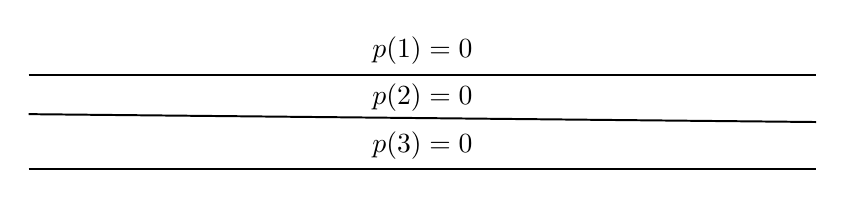
\begin{tikzpicture}
            \draw[line width=0.25mm] (0,0) -- (10,0)  node[above,xshift=-5cm] {$p(1)=0$};
            \draw[line width=0.25mm] (0,-0.5) -- (10.0,-0.6) node[above,xshift=-5cm] {$p(2)=0$};
            \draw[line width=0.25mm] (0,-1.2) -- (10.0,-1.2) node[above,xshift=-5cm] {$p(3)=0$};
        \end{tikzpicture}

        \pagebreak


        2. Give examples where the sequence alternates between $0$ and $1$. 

        No overlapping with previous index request (pairwise compatible)


        Alternates between overlapping with the first request and not overlapping the first request. 

        \begin{tikzpicture}
            \draw[line width=0.25mm] (0,0) -- (5,0)  node[above,xshift=-2.5cm] {$p(1)=0$};
            \draw[line width=0.25mm] (6,-1.0) -- (8,-1.0) node[above,xshift=-1cm] {$p(2)=1$};
            \draw[line width=0.25mm] (4,-2.0) -- (9,-2.0) node[above,xshift=-2.5cm] {$p(3)=0$};
            \draw[line width=0.25mm] (6,-3.0) -- (10,-3.0) node[above,xshift=-2cm] {$p(4)=1$};
            \draw[line width=0.25mm] (4,-4.0) -- (11.0,-4.0) node[above,xshift=-3.5cm] {$p(5)=0$};
            \draw[line width=0.25mm] (6,-5.0) -- (10,-5.0) node[above,xshift=-2cm] {$p(6)=1$};
            \draw[line width=0.25mm] (4,-6.0) -- (11.0,-6.0) node[above,xshift=-3.5cm] {$p(7)=0$};
        \end{tikzpicture}

    
        3. Give examples where the sequence has the form $0,1,...,n-1$

        \begin{tikzpicture}
            \draw[line width=0.25mm] (0,0) -- (3,0)  node[above,xshift=-1.5cm] {$p(1)=0$};
            \draw[line width=0.25mm] (3.1,-1.0) -- (6.0,-1.0) node[above,xshift=-1.45cm] {$p(2)=1$};
            \draw[line width=0.25mm] (6.1,-2.0) -- (9.0,-2.0) node[above,xshift=-1.45cm] {$p(3)=2$};
            \draw[line width=0.25mm] (9.1,-3.0) -- (12.0,-3.0) node[above,xshift=-1.45cm] {$p(4)=3$};
        \end{tikzpicture}

        And so forth, and we will get that $p(n)=n-1$.

        Another example is (in order) :

        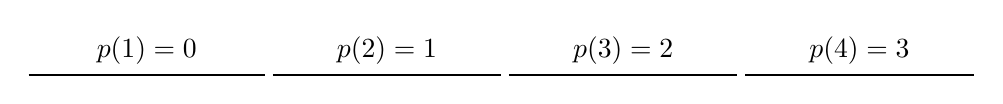
\begin{tikzpicture}
            \draw[line width=0.25mm] (0,0) -- (3,0)  node[above,xshift=-1.5cm] {$p(1)=0$};
            \draw[line width=0.25mm] (3.1,-0.0) -- (6.0,-0.0) node[above,xshift=-1.45cm] {$p(2)=1$};
            \draw[line width=0.25mm] (6.1,-0.0) -- (9.0,-0.0) node[above,xshift=-1.45cm] {$p(3)=2$};
            \draw[line width=0.25mm] (9.1,-0.0) -- (12.0,-0.0) node[above,xshift=-1.45cm] {$p(4)=3$};
        \end{tikzpicture}

        and so forth...
        






        

    

    




    \end{homeworkProblem}

       



    \end{document}
    